% Copyright (C) 2010 Thomas L. Kula
% All Rights Reserved
%
% See the file LICENSE for license terms.
\documentclass[12pt]{article}
\usepackage{graphicx}
\usepackage{rotating}
\usepackage{fix-cm}
\usepackage{multirow}
\setlength{\paperwidth}{5.5in}
\setlength{\paperheight}{8.5in}
\setlength{\textheight}{7.45in}
\setlength{\topmargin}{-1.0in}
\setlength{\oddsidemargin}{-0.5in}
\setlength{\evensidemargin}{-0.5in}
\setlength{\textwidth}{4.0in}
\setlength{\parindent}{0in}
\setlength{\parskip}{3mm}
\usepackage[print]{booklet} \nofiles
\source{\magstep0}{5.5in}{8.5in}
\target{\magstep0}{11in}{8.5in}
\setpdftargetpages
\pagestyle{empty}
\begin{document}


\begin{center}
{\fontsize{36}{48}\selectfont \textsc{Haiku a Day }}
\end{center}

\vspace*{3.5cm}

{\fontsize{20}{40}\selectfont 


So much left to do

So little time to do it

Buckle down to work

}

\vspace*{5.0cm}
\begin{center}
{\large{Issue 65: November 2010}} \\[5mm]
{\fontsize{8}{8}\selectfont  \textsc{ St. Joshua Norton Press }} \\[1mm]
{\fontsize{6}{6}\selectfont Mathom House in Midtown \textbar The People's Republic of Ames }
\end{center}


\newpage

It's the end of the year, and a busy time. While I've enjoyed
Thanksgiving and the Detroit Urban Craft Fair, and will enjoy
DIYpsi, the Krampus Ball and the Krampus edition of Elbow
Deep and look forward to seeing family at Christmas, man, I
can't wait for 2011 to be here.

--- Thomas

http://kula.tproa.net/had/ \\
kula@tproa.net

Download this and previous HADs at the website, so you can
print out your own (DIY, yeah!) or if you want me to send
you one, send me your address, and maybe a stamp if you
are feeling nice. Or send me something you've made ---
trades always appreciated, postcards are nice too.

\vfill

1 November 2010

A trumpet sounds out \\
Faintly, behind a window \\
I can hear its call

2 November 2010

A grate in the curb \\
Hiding fantastic secrets \\
In its murky depths

\newpage

3 November 2010

A dense pancake \\
Flat in the street, covering \\
Places I can't go

4 November 2010

Standing in the wind \\
Bravely pointing out the way \\
I salute you, sign!

5 November 2010

An ominous eye \\
Balefully glaring in red \\
Warns you not to go

6 November 2010

Cold morning, early \\
Pastel clouds spray through the sky \\
Happy with the Sun

7 November 2010

Gumption lost, naps win \\
Warm bed a powerful draw \\
To hide from the world

8 November 2010

Constant confounding \\
The knot that's untyable \\
What did I sleep on?

9 November 2010

Haze glowing brightly \\
An alien glow abounds \\
With time, burns away


\newpage

10 November 2010

Old maps tell stories \\
The lines become story arcs \\
Place a dialog

11 November 2010

Where did you come from? \\
Bombastic sneeze, blowing up \\
A small hurricane

12 November 2010

Forced into a store \\
Errands expose me to cheer \\
I hate holidays

13 November 2010

O happy jingle! \\
Go to pizza! To pizza! \\
The oven is done.

14 November 2010

While you must balance \\
In some sloth, serenity \\
The sweet lazy joy

15 November 2010

Slow and steady wins \\
But life often ends up here: \\
Quick burst --- then nothing

16 November 2010

The patter of rain \\
Syncopates with the dryers \\
Wet, dry, together


\newpage

17 November 2010

Does it overflow? \\
Or, it half empty, half full \\
The cup, confounding

18 November 2010

The fork, metal hand \\
Stabbing everything in sight \\
Tines: two, three or four

19 November 2010

The knife is edgy \\
Small, large, curvy or pointy \\
Ready to cut you

20 November 2010

The spoon's graceful arcs \\
A concavity holding \\
Nestled in the bowl

21 November 2010

Forget not the plate! \\
Brave, strong, holding up in need \\
It gives you plenty

22 November 2010

Holidays looming \\
I'm so glad for a short week \\
Plenty of napping

23 November 2010

Awash with good food \\
Thanksgiving ideas erupt \\
Tasty times to come


\newpage

24 November 2010

Why work today? \\
Holidays, nothing gets done \\
Just biding my time

25 November 2010

Lord of the Rings Day \\
Food, videos and napping \\
A glorious time

26 November 2010

Amazing movies \\
Available anytime \\
I love the future

27 November 2010

Outside, biting wind \\
Against the window it slams \\
Warmth keeps it at bay

28 November 2010

Details unnoticed \\
A corner of a painting \\
Shines in a new light

29 November 2010

Awake way too late \\
Tomorrow a tired day \\
But it awakes joy

30 November 2010

In warmth, happiness \\
The faint breath of the furnace \\
Lulling me to sleep


\newpage

\begin{center}
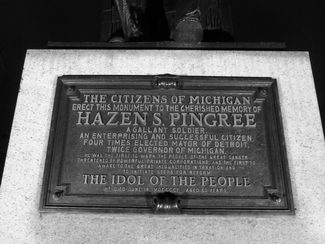
\includegraphics{monument.png}

Pingree Monument, Grand Circus, Detroit \\
{\em They don't make `em like this anymore}

\small{{\tt kula.tproa.net/photos/2010/ducf5/ }}
\end{center}


\newpage

\thispagestyle{empty}
\vspace*{14cm}
\begin{sideways}
\Large{Thomas L. Kula}
\end{sideways}
\begin{sideways}
\Large{PO Box 980461}
\end{sideways}
\begin{sideways}
\Large{Ypsilanti MI 48198}
\end{sideways}


\end{document}


